%#!make IN201503.dvi
\documentclass[technicalreport]{ieicej}
\usepackage[dvipdfmx]{graphicx}
% For URL support
\usepackage{url}


%======================================================================
% プリアンブル
%======================================================================
% 表示位置の修正
\hoffset -8mm
\voffset -8mm

%% 行間
\def\baselinestretch{0.95}

% ハイフネーションを修正
\hyphenation{net-works}

% 縦に並べた図の間の基準となるスペース
\newlength\figuresep
\setlength{\figuresep}{0.3\floatsep}

% enumerate環境のインデントを変更
\makeatletter
\renewenvironment{enumerate}
  {%
   \ifnum \@enumdepth >3\relax\@toodeep\else
    \advance\@enumdepth\@ne
    \edef\@enumctr{enum\romannumeral\the\@enumdepth}%
    \list{\csname label\@enumctr\endcsname}{%
    \leftmargin1.5zw
    \labelsep1zw
    \labelwidth\z@
    \itemindent2zw
    \listparindent1zw
    \topsep\z@\parsep\z@\partopsep\z@\itemsep\z@
    \usecounter{\@enumctr}%
    \def\makelabel##1{\hss\llap{##1}}}%
   \fi}{\endlist}
\makeatother

%----------------------------------------------------------------------
% タイトル
%----------------------------------------------------------------------
%和文タイトル
\jtitle{WLANとZigBeeの共存に向けたAP-Assisted CTS-Blockingの評価}
%英文タイトル
\etitle{Evaluation of an AP-Assisted CTS-Blocking aiming at co-existence of WLAN and ZigBee}

%著者たち
%E-mail掲載希望の場合は[ ]に含める
\authorlist{
 \authorentry{佐伯 良光}{Yoshiteru Saeki}{Kyu}
 \authorentry{石田 繁巳}{Shigemi Ishida}{Kyu}
 \authorentry{田頭 茂明}{Shigeaki Tagashira}{Kan}
 \authorentry{福田 晃}{Akira Fukuda}{Kyu}
}
\affiliate[Kyu]%
{九州大学大学院システム情報科学府・研究院 〒819--0395 福岡市西区元岡744番地}%
{Guraduate School/Faculty of Information Science and Electrical Engineering,
Kyushu University%
%Motooka 744, Nishi-ku, Fukuoka,
%819--0395 Japan
}
\affiliate[Kan]%
{関西大学総合情報学部 〒569--1095 大阪府高槻市霊仙寺町2-1-1}%
{Faculty of Informatics, 
Kansai University%
%2-1-1 Ryozenji-cho, Takatsuki-shi, OSAKA,
%569--1095 Japan
}

%======================================================================
% テキスト開始
%======================================================================
\begin{document}

%----------------------------------------------------------------------
% 和文あらまし
%----------------------------------------------------------------------
% 500字程度
\begin{jabstract}
 筆者らは,同周波数帯を利用するWLANとZigBeeの同空間における共存に向けて容易に構
 築可能な衝突回避システムの研究を行っている.
 衝突回避システムにおいては通信の公平性確保の為,システム改変に多くの制約がある.
 このような観点から,既存の方式を活用する,パケットを二重送信する等,システム改変の
 制約にあたらないシンプルなシステム構築が重要となる.
 本稿ではZigBeeネットワークが無線LAN(WLAN)から受ける干渉の影響を軽減するための
 AP-Assisted CTS-Blocking(AA CTS-Blocking)を示す.
 AA CTS-BlockingはRTS/CTS方式を応用することでWLANの通信を抑制し,ZigBee通信と
 WLAN通信の衝突を回避させる.
 AA CTS-Blockingを用いた衝突回避システムを実装し,実証評価を通じてZigBeeネットワーク
 の通信エラー率を評価する.
\end{jabstract}

%和文キーワード
\begin{jkeyword}
 WLAN,ZigBee,衝突回避,AA CTS-Blocking
 Webサービス.
\end{jkeyword}

%----------------------------------------------------------------------
% 英文あらまし
%----------------------------------------------------------------------
% 100 words程度
\begin{eabstract}
 The authors readily configured toward the coexistence in the same space of the WLAN and ZigBee utilizing the same frequency band
 You are conducting research on dating possible collision avoidance system .
 Because in the collision avoidance system of fairness ensure communication , there are a number of constraints on the system modification .
 Etc. from this point of view , to use the existing access control system , to double the header packet ,
 Simple system construction that does not hit the constraint is important .
 This paper is to reduce the effects of interference ZigBee network receives from a wireless LAN (WLAN) is
 AP-Assisted CTS-Blocking I show the (AA CTS-Blocking).
 AA CTS-Blocking inhibits communication of the WLAN by applying the RTS / CTS method , a ZigBee communication
 I to avoid the collision of WLAN communication .
 Implements the collision avoidance system using AA CTS-Blocking, and ZigBee network through empirical evaluation
 I evaluate the communication error rate .
\end{eabstract}

%英文キーワード
\begin{ekeyword}
 Wireless-Local Area Network (WLAN),ZigBee,Collision Avoidance,Access Point-Assisted 
 Clear to Send-Blocking (AA CTS-Blocking)
\end{ekeyword}

\maketitle

%======================================================================
% 本文ここから
%======================================================================
\section{はじめに}
\label{sec:intro}

GPS(Global Positioning System)モジュールを搭載したスマートフォンなどの
端末の普及とともに,ユーザの位置に応じて目的地への案内や周辺情報の提供な
どを行う「位置情報サービス」が広がりを見せている.
これらの位置情報サービスはGPSを用いるために主に屋外での利用を想定してい
る.
位置情報サービスを屋内へと拡大するためには屋内で利用可能な測位技術が重要
となる.
このため,屋内測位技術に関する多くの研究開発が進められている.

筆者らは,イベント会場や工事現場などにおいて利用するための一時的な屋内位
置情報サービスの実現に向けて,アドホック測位ネットワーク
\cite{izumi13:awpn_acc_imprv}の研究を行っている.
アドホック測位ネットワークは,無線LANアクセスポイント(AP)間の通信によっ
てネットワークを構築する「無線LANメッシュネットワーク技術」
\cite{sakata06:ad-hoc_wlan_mesh}を用いた測位システムである.
測位に必要となる受信電波強度(RSSI)情報を無線LANメッシュネットワークを
通じて転送することで,無線LAN AP及び測位計算を行うサーバを設置するだけで
測位システムを構築できる.

一時的な位置情報サービスの実現に向けては,測位システムに加えてユーザ端末
へのアプリケーション導入の容易さも重要となる.
屋内位置情報サービスはすでに実用化されている例も報告されているが,これら
のサービスにおいてはユーザが専用のアプリケーションをインストールして利用
することが想定されている.
展示会などのイベント会場でこのような屋内位置情報サービスを一時的に利用す
る場合を考えると,ユーザが一時的にアプリケーションを導入する必要が生じる
ため,サービス利用への大きな障壁となる.

アプリケーション導入に対するユーザの負担軽減に向けて,本研究では位置情報
サービスをWebサービスとして提供するアプローチをとる.
ユーザ端末の位置に応じた動的なWebコンテンツを配信することで位置情報サー
ビスを実現する.
ユーザは無線LAN端末からWebサーバにアクセスするだけで位置情報サービスを利
用することが可能となるため,災害時などユーザが事前準備を行うことが困難な
場合への応用も期待できる.

アドホック測位ネットワークは無線LAN AP間のマルチホップ通信によって形成さ
れているため,アプリケーションレス位置情報Webサービスの実現に向けては通
信負荷の分散が重要となる.
これまでにも無線LANを用いた屋内測位技術に関する多くの研究が行われている
が,筆者らの調査の範囲内では制約のあるネットワークにおける位置情報サービ
スの提供に向けた検討は行われていない.

本稿では,アドホック測位ネットワーク上で自律分散動作するアプリケーション
レス測位システムを示す.
アプリケーションレス測位システムは,アドホック測位ネットワークを構成する
各無線LAN AP内のWebサーバ,RSSI受信サーバ,RSSI観測サーバの3つのサーバに
よって構成される.
ユーザ端末が接続されているAP内のサーバを中心に,各AP内の各サーバを自律的
に動作させることによって通信負荷を分散させる.

本稿の構成は以下の通りである.
\ref{sec:wlan_pos}ではアドホック測位ネットワークについて述べ,位置情報サー
ビスをWebサービスとして実現する際の課題について述べる.
\ref{sec:app-less}ではアドホック測位ネットワーク上におけるアプリケーション
レス測位システムを示す.
\ref{sec:imple}では無線LANメッシュノードを用いたアプリケーションレス測位
システムの実装について述べ,
\ref{sec:eval}において基本性能評価を行う.
最後に\ref{sec:concl}でまとめとする.

%----------------------------------------------------------------------
\section{アドホック測位ネットワーク}
\label{sec:wlan_pos}

\begin{figure}[bt]
 \centering
 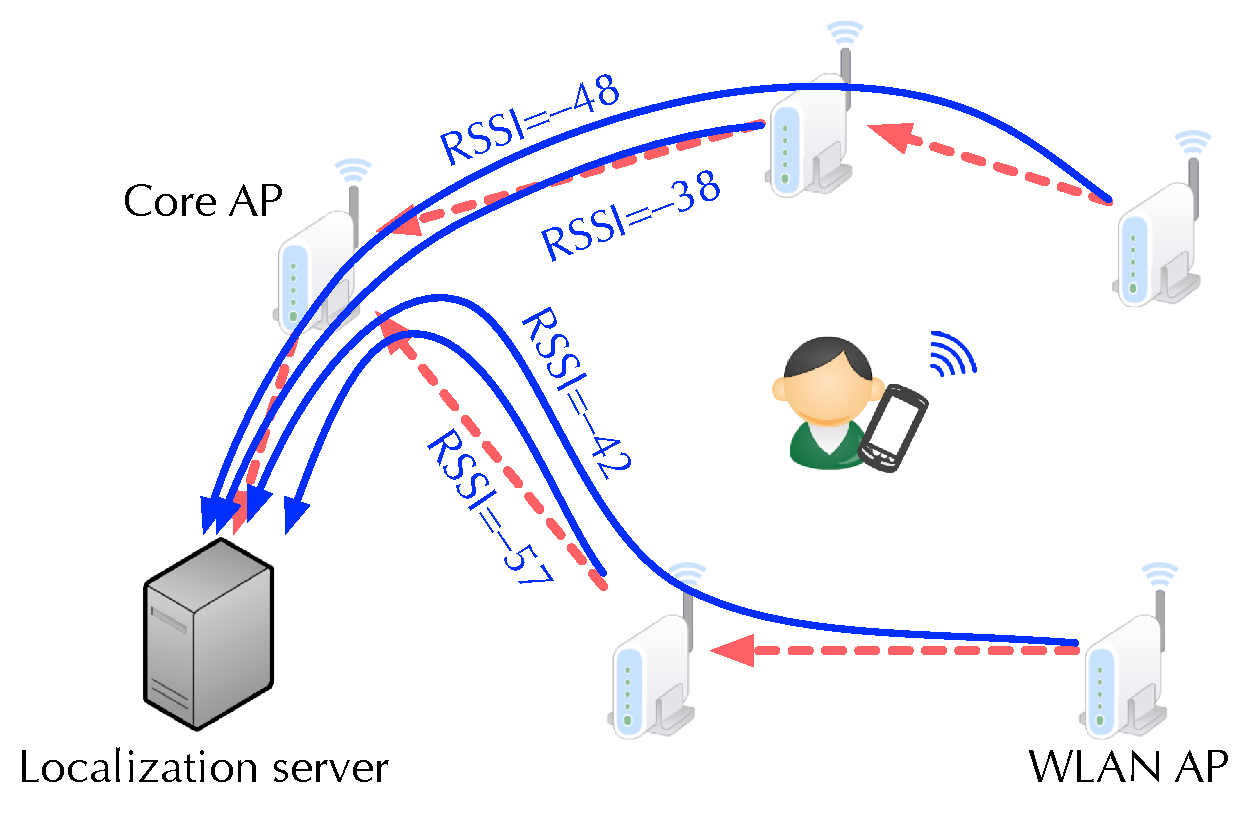
\includegraphics[width=0.9\columnwidth]{figure/awpn_overview.eps}
 \caption{アドホック測位ネットワークの概要}
 \label{fig:adhoc}
\end{figure}

アドホック測位ネットワークは,無線LANメッシュネットワーク技術によって形
成された無線LAN AP間ネットワークを用いて無線LAN端末の測位を行うシステム
である.
\figurename~\ref{fig:adhoc}にアドホック測位ネットワークの概要を示す.
アドホック測位ネットワークは,複数台の無線LAN APと測位サーバとから構成さ
れる.
測位対象エリアに無線LAN APを設置し,無線LAN APの1つに測位サーバを接続す
ると,無線LAN AP間のマルチホップ通信によりネットワークが自動的に形成され
る.
測位対象エリア内でユーザの無線LAN端末が信号を発すると,ユーザ端末の信号
を検出した無線LAN APは検出した信号のRSSIと送信元アドレスをRSSI情報として
測位サーバに送信する.
測位サーバは複数の無線LAN APから受信したRSSI情報と各無線LAN APの座標情報
を用いて,ユーザ端末の位置を多辺測量法などにより算出する.

アドホック測位ネットワーク上でアプリケーションを用いずにユーザに位置情報
サービスを提供するため,Webサービスとして位置情報サービスを提供する.
アドホック測位ネットワーク上では測位サーバにおいて測位計算が行われるため,
Webサーバを測位サーバと同じ計算機上に構築し,測位結果に応じてWebコンテン
ツを変更することで位置情報サービスを実現する.

位置情報サービスを利用する場合,ユーザは無線LAN端末で無線LAN APの1つに接
続してWebサーバにアクセスする.
各無線LAN APはユーザ端末がWebアクセス時に発した信号を検出するとRSSI情報
を測位サーバに送信し,測位サーバにおいてユーザ端末の測位計算が行われる.
Webサーバは測位サーバの計算終了を待機し,ユーザ位置を表示する地図など,
位置情報サービスページをユーザ端末に返却する.
ユーザ位置などを自動的に更新するため,Webページに埋め込まれたスクリプト
プログラムを利用して定期的にWebアクセスを発生させ,Webコンテンツを更新す
る.

このようなWebサービスを実現する上では,ユーザビリティの観点からユーザが
WebアクセスをしてからWebコンテンツが返却されるまでの応答時間を短くするこ
とが望ましい.
これに向けて通信負荷を分散させることが求められる.
アドホック測位ネットワークは無線LAN AP間のマルチホップ通信によって形成さ
れているため,測位サーバ付近の無線LAN APでは多数の無線LAN APからの情報を
転送する必要があり,通信が混雑する.
また,1台のユーザ端末に対して複数台の無線LAN APがRSSI情報を送信すること
を考えるとユーザ端末数の増加とともに通信量が大きく増加する.
Webの応答時間というユーザビリティの観点だけでなく,利用者数の増加に対応
するためにも測位サーバ付近での通信負荷の集中を避ける必要がある.

無線LANを用いた屋内測位に関しては,測位精度の向上や測位環境の容易な構築
に関する研究を中心として多くの研究が行われている
\cite{sun05:sig_proc_pos}.
測位精度の向上に関しては,観測されたRSSI情報からの端末位置推定において,
RSSI自体の時間変動やバラツキ,無線LANモジュールのベンダーの違いによる影
響を考慮する手法\cite{kaemarungsi12:wlan_rssi_analysis},
複数端末で協調させる測位計算手法\cite{wymeersch09:coop_loc},
高精度化に向けたボトルネックを明確化するための精度・頑健性・環境構築コス
トのトレードオフ解析\cite{prasithsangaree02:indoor_wlan_loc}
などが報告されている.
また,無線センサネットワーク分野においても,時空間的な相関を考慮した測位
計算手法\cite{blumrosen13:rssi_track_wsn}など,無線LAN測位に応用すること
ができる測位精度向上手法が報告されている.
本研究においてもこのような手法を用いて測位計算を行うことで,測位精度の向
上が可能である.

測位環境の容易な構築に関しては,
アドホック測位ネットワークと同様に無線LAN APで観測した信号を用いて測位す
る手法\cite{ganu04:infra_loc_wlan},
無線LAN APなど環境構築の際に導入するノード数を最小化する手法
\cite{krishnan04:lease},
RSSI特徴量の領域で端末測位を行うことでRSSI特徴量と物理的な位置の対応付け
に要するコストを削減する手法\cite{yang12:locate_finger},
モバイル端末のGPSと組み合わせるなどしてアクセスポイントの座標を自動的に
算出する手法
\cite{chintalapudi10:indoor_loc_nopain,lim10:zero-config_loc}
などが報告されている.
測位環境の構築に関して多くの報告がある一方で,ユーザ端末への位置情報サー
ビスの提供方法については検討がなされておらず,ユーザ端末へのアプリケーショ
ンの導入が暗黙的に想定されている.
また,アドホック測位ネットワークのように通信帯域に制約がある場合の位置情
報サービスの提供に向けた検討は行われていない.

%----------------------------------------------------------------------
\section{AA-CTS Blocking}
\label{sec:aa_cts}

前節で述べたように,WLANとZigBeeの共存に向けた衝突回避システムの実現に向
けてはさせることが求められる.
ここで,ユーザ端末の信号を検出する無線LAN APがユーザ端末と物理的に近い距
離にあることに着目する.
ユーザ端末の信号検出の可否は,通信の衝突を考慮しなければ端末からの距離に
応じた信号減衰によって決まるため,ユーザ端末から十分に離れた距離にある無
線LAN APは信号を検出することができない.
ユーザ端末の信号を検出した無線LAN AP間のみで通信を行えば,アドホック測位
ネットワーク上でのホップ数が少なく,他の無線LAN APの通信に与える影響を低
減できると考えられる.

本節では,このような考えに基づいて設計されたアプリケーションレス測位シス
テムを示す.
本システムでは,位置情報Webサービスを実現する測位サーバとWebサーバをユー
ザ端末の接続先AP上で動作させる.
これにより通信を物理的に近い無線LAN AP間にとどめ,ユーザ端末の物理的な分
散に応じて複数のユーザ端末の通信を分散させる.

%--------------------------------------------------
\subsection{アプリケーションレス測位システムの概要}

本システムでは,周辺にあるWLAN APからCTSフレームを送信させてCTS-Blockingを実現する.
これにより,WLAN通信の一時的ブロックによる効率的なZigBee通信の実現を目指す.
また,RTSを送信するAPの選択については,APから取得できる情報を基に最適なAP選択アルゴリズムを考慮する.

図\ref{fig:3_01}に,AA CTS-Blockingシステムの概要を示す.
本システムは,環境内に配置された複数のZigBeeノード及びZigBee基地局,制御PCから構成される.
ZigBee基地局と制御PCは有線接続されている.

制御PCでは,周囲に存在するWLAN APのビーコンフレームを受信し,チャネル,受信信号強度(RSSI)を収集する.
ZigBeeの通信を開始する場合,周囲のAPの1つを選択して制御PCからRTSフレームを送信する.
選択されたAPはRTSフレームを受信すると周囲のWLAN端末に対してCTSフレームを送信する.
制御PCはAPからのCTSフレームを受信するとZigBee基地局を用いてZigBeeノードとの通信を開始する.
WLAN APは,そのAPが提供するWLANネットワークに参加していない端末からのRTSフレームに対しても
CTSフレームを返答するため,制御PCでは任意のAPを選択することができる.

\begin{figure}[bt]
 \centering
 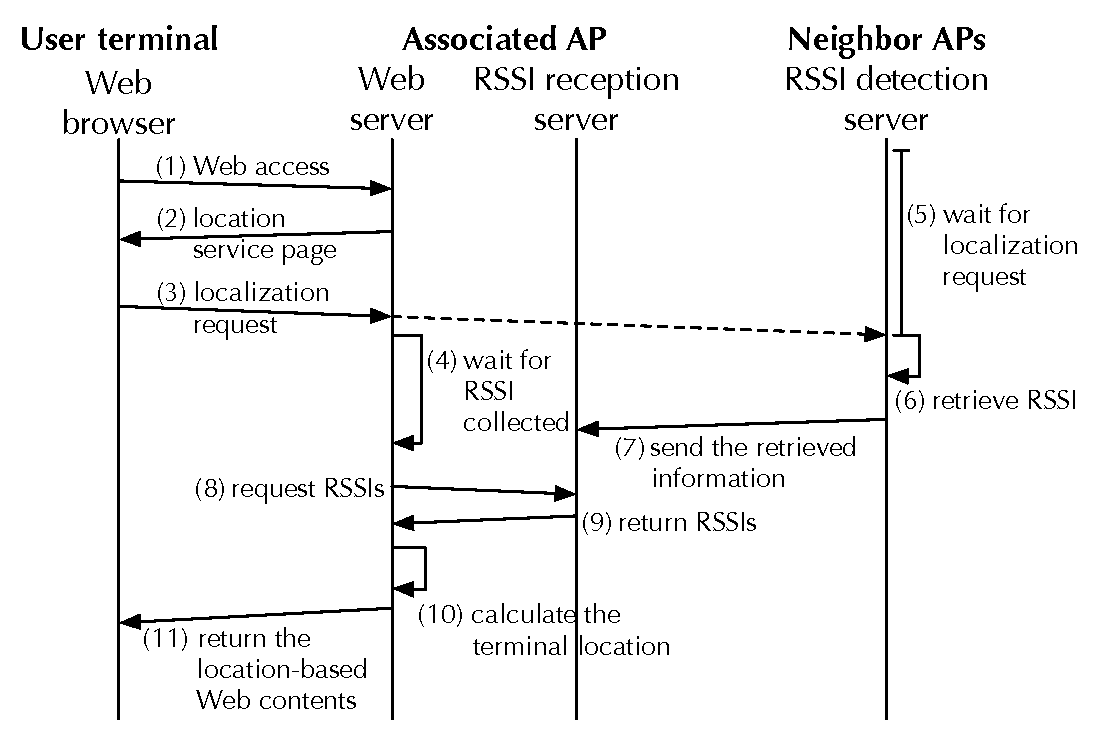
\includegraphics[width=\columnwidth]{figure/sequence.eps}
 \caption{AA CTS-blockingシステムの通信シーケンス}
 \label{fig:sequence}
\end{figure}

\figurename~\ref{fig:sequence}にAA CTS-blockingシステムの通信シーケンスを示す.
まず,ブロックしたいWLAN通信を構築する無線LAN APのチャネルを設定する.

\noindent
(1)~制御PCは設定されたチャネルを利用しているAPの中から1つのAPを選択する.

\noindent
(2)~制御PCはAPに向けてRTSフレームを送信する.

\noindent
(3)~RTSフレームを受信したAPはCTSを返却し,同時に周囲の接続WLAN端末に向
けてCTSフレームをブロードキャストする.

\noindent
(4)~制御PCはAPからのCTSフレームを受信するまで待機する

%(4)'~CTSフレームを受信せず一定時間が経過した場合,タイムアウトし(2)へ戻る.
\noindent
(5)~制御PCはAPから返却されたCTSフレームを受信すると,有線接続されたZigBee
基地局に向けて通信開始信号を送信する.

\noindent
(6)~この時,制御PCはCTS-Blockingタイマを起動させる.

\noindent
(7)~通信開始信号を検出したZigBee基地局は,sleep状態から復帰し.active状態へ
移行する.

\noindent
(8)~active状態となったZigBee基地局は,周囲のZigBeeノードへ送信要求フレームを
ブロードキャストする.

\noindent
(9)~この時,ZigBee基地局はActive ZigBee-Commタイマを起動させ,listen状態へ移行する.

\noindent
(10)~送信要求フレームを受け取った周囲のZigBeeノードは,standby状態から
transmit状態へと移行する.

\noindent
(11)~transmit状態へと移行したZigBeeノードは,それぞれのノードに設定された
固有のガード時間だけ待ってZigBee基地局へデータフレームを返信する.

\noindent
(12)~送信が完了したら,ZigBeeノードはtransmit状態からstandby状態へ移行する.

\noindent
(13)~listen状態となったZigBee基地局は,周囲のZigBeeノードから返信されるデータ
フレームを受信するまで待機する.

\noindent
(14)~周囲のZigBeeノードからデータフレームを受信したら,ZigBee基地局はlisten状態
からdisplay状態へと移行する.

\noindent
(15)~display状態へと移行したZigBee基地局は,有線接続された制御PCにデータ
フレームを転送する.

\noindent
(16)~転送されたデータフレームを受け取った制御PCは,自身のコンソール上にデータ
フレームの中身を表示する.

\noindent
(17)~転送完了後,ZigBee基地局はdisplay状態からすぐにlisten状態へと移行し,(13)へ
戻る.

\noindent
(18)~Active ZigBee-Commタイマが終了すると,ZigBee基地局はlisten/display状態から
すぐにsleep状態へと移行し,受信待機を解除する.

\noindent
(19)~CTS-Blockingタイマが終了すると,AA CTS-Blockingは終了となる.

制御用通信による通信帯域の消費を低減するため,アプリケーションレス測位シ
ステムでは各無線LAN AP内のサーバを自律的に動作させる.
以下では各機器の動作の詳細を示す.

%--------------------------------------------------
\subsection{Webサーバ}
\label{ssec:design_web_server}

Webサーバは,ユーザ端末への位置情報Webサービスページの提供と,ユーザ端末
からの測位要求による測位計算を行う.

\begin{figure}[bt]
 \centering
 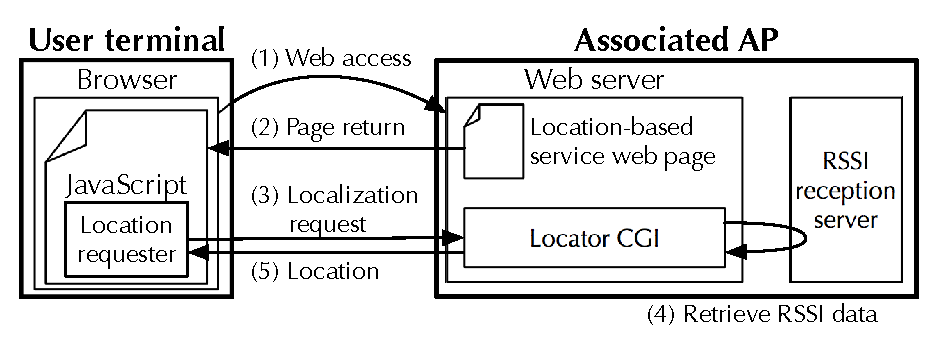
\includegraphics[width=\columnwidth]{figure/web_server.eps}
 \caption{Webサーバの動作}
 \label{fig:web_server}
\end{figure}

\figurename~\ref{fig:web_server}にWebサーバの動作を示す.
ユーザ端末のブラウザがWebサーバにアクセスすると,Webサーバは測位要求を行
うJavaScriptプログラムが埋め込まれたWebページを返却する.
測位要求プログラムはWebサーバ上の測位CGIにアクセスし,測位を要求する.
Webサーバ上の測位CGIは,アクセス元のIPアドレスを取得し,IPアドレスをキー
としてRSSI受信サーバから測位計算に必要となるRSSI情報を取得する.
取得したRSSI情報を用いて測位計算を行い,測位結果をJSON形式で記述してユー
ザ端末に返却する.
受信した測位結果を用いて測位要求プログラムはWebページを更新する.

測位CGIにおいてRSSI情報を取得する際には,測位CGIへのアクセスに関するRSSI
情報が収集されるまで待機することが望ましい.
この場合,各無線LAN APを自律的に動作させるためには測位CGIにおけるRSSI情
報取得までの待ち時間を自律的に決定する必要がある.
測位CGIの待機時間は,RSSI情報の受信に要する時間から決定できる.
詳細については\ref{ssec:rssi_rx_time}において述べる.


ユーザ端末は自動的に周囲の無線LAN APに接続されるため,ユーザが接続先のAP
を認識していないことが予想される.
この場合にはユーザがブラウザを使用した際に接続先AP上のWebサーバに自動的
に接続することが必要となる.
このような自動接続は,RADIUSサーバを用いたリダイレクトやファイヤウォール
を用いた転送などによって実現できると考えている.

%--------------------------------------------------
\subsection{RSSI受信サーバ}

\begin{figure}[bt]
 \centering
 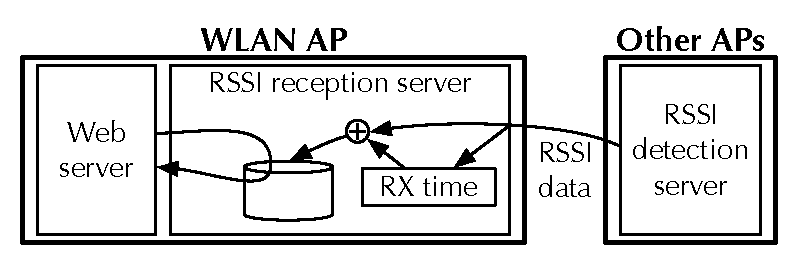
\includegraphics[width=0.8\columnwidth]{figure/rssi_rx_server.eps}
 \caption{RSSI受信サーバの動作}
 \label{fig:rssi_rx_server}
\end{figure}

\figurename~\ref{fig:rssi_rx_server}にRSSI受信サーバの動作を示す.
RSSI受信サーバは,RSSI観測サーバより送信されたRSSI情報を受信して蓄積し,
Webサーバ上の測位CGIに提供する.
このとき,測位CGIがユーザ端末に関する最新のRSSI情報を特定できるように,
RSSI情報の受信時刻も同時に蓄積する.
測位計算では各ユーザ端末に関する最新のRSSI情報が使用されるため,RSSI受信
サーバは一定個数のRSSI情報を蓄積して古いRSSI情報は破棄する.
蓄積するRSSI情報の個数は,無線LAN APのリソース(メモリ・ディスク)の大き
さから決定する.

RSSI受信サーバはRSSI観測サーバからのRSSI情報を蓄積するだけの機能を担って
おり,同一AP内の他のサーバ,他の無線LAN APに影響されず自律的に動作する.

%--------------------------------------------------
\subsection{RSSI観測サーバ}
\label{ssec:rssi_detect}

\begin{figure}[bt]
 \centering
 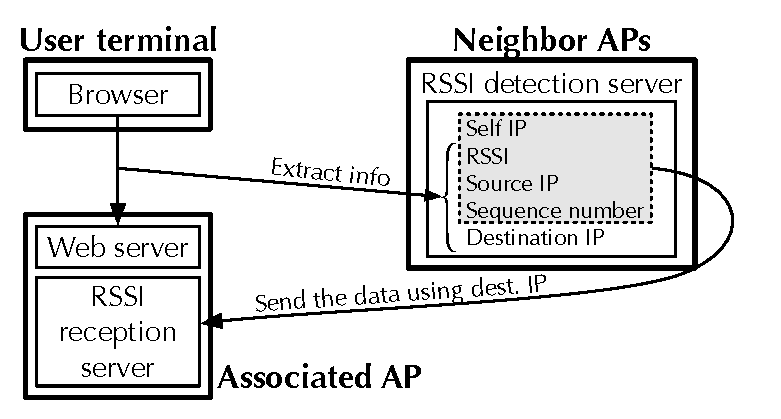
\includegraphics[width=0.9\columnwidth]{figure/rssi_detect_server.eps}
 \caption{RSSI観測サーバの動作}
 \label{fig:rssi_detect_server}
\end{figure}

\figurename~\ref{fig:rssi_detect_server}にRSSI観測サーバの動作を示す.
RSSI観測サーバはユーザ端末から発せられる測位要求を監視し,測位要求を検出
した場合にはその測位要求を受信して以下の4つの情報を収集する.
\begin{enumerate}
 \item RSSI

       ユーザ端末の測位に用いられる.
       無線LANモジュールから取得できる.

 \item 送信元IPアドレス

       測位CGIがユーザ端末を識別するために用いられる.
       測位要求は測位CGIへのアクセスを行うIPパケットであるから,IPヘッダ
       から取得できる.

 \item シーケンス番号

       測位CGIが最新のRSSI情報を特定するため,及び同一の測位要求を特定す
       るために用いられる.
       IEEE\,802.11 MACによる再送があった場合にも測位要求を区別できるよ
       うにするため,IEEE\,802.11 MACヘッダの\texttt{Frame Control}フィー
       ルドに含まれる\texttt{Sequence Control}フィールドの値をシーケンス
       番号として用いる.

 \item 宛先IPアドレス

       RSSI観測サーバがRSSIを送信する宛先を特定するために用いられる.
       IPヘッダから取得できる.
\end{enumerate}

これらの情報のうち,RSSI,送信元IPアドレス,シーケンス番号をまとめてRSSI
情報とし,宛先IPアドレスのRSSI受信サーバに対して送信する.
測位要求の宛先IPアドレスは,ユーザ端末の接続先APであるため,1台のユーザ
端末から発せられた測位要求に関するRSSI情報は端末接続先APのRSSI受信サーバ
に集まることとなる.

RSSI観測サーバは,受信した測位要求のみに基づいて自律的に動作する.

%----------------------------------------------------------------------
\section{実装}
\label{sec:imple}

\begin{table}[tb]
 \footnotesize
 \centering
 \caption{PCWL-0100の主要諸元(抜粋)\cite{picocela:pcwl-0100}}
 \label{tab:pcwl-0100_spec}
 \begin{tabular}{lp{4.8cm}}\Hline
  見通し内中継回線到達距離 & 約150\,m(伝搬環境によって変化) \\
  中継回線出力 & 16\,dBm \\
  アクセス回線出力 & 16\,dBm \\
  アクセス回線無線IF & IEEE\,802.11b/g対応 \\
  中継回線無線IF & 2つ内蔵(アクセス回線無線IFとは別)
      $5.15\sim5.35$\,GHz \\
  本体サイズ & 幅142\,mm$\times$縦118\,mm$\times$奥行き39\,mm\\ \Hline
 \end{tabular}
\end{table}

\ref{sec:app-less}で示したアプリケーションレス測位システムの動作の実証と
基本性能の評価に向けて,無線LANメッシュノードを用いて本システムを実装し
た.
無線LANメッシュノードとしては,PicoCELA社の
PCWL-0100~\cite{picocela:pcwl-0100}(以下PCWLと表記)を用いた.
\tablename~\ref{tab:pcwl-0100_spec}にPCWLの主要な諸元を示す.
PCWLは中継機能を有した無線LAN APであり,PCWL間のマルチホップ通信により自
動的にネットワークを構築することができる.

PCWL内ではLinuxが動作しており,このLinux上にWebサーバ,RSSI受信サーバ,
RSSI観測サーバを実装した.

Webサーバは,オープンソースのHTTPサーバであるthttpd~\cite{acme:thttpd}を
用い,測位CGIはC言語で実装した.
測位CGIとRSSI受信サーバとの通信は,同一のAP内における通信であること,デー
タ送受信の方向が一定であることから,各サーバの自律性を高めるために共有メ
モリを用いた.

RSSI受信サーバ及びRSSI観測サーバはC言語で実装した.
RSSI観測サーバにおいては,モニターモードの無線LANインタフェースを用いて
Radiotapヘッダが付加されたIEEE\,802.11 MACフレームを受信し,
\ref{ssec:rssi_detect}で示したRSSI,送信元IPアドレス,シーケンス番号,宛
先IPアドレスの4つの情報を取得した.
RSSI受信サーバとRSSI観測サーバ間の通信はTCP通信を用いた.

\begin{figure}[bt]
 \centering
 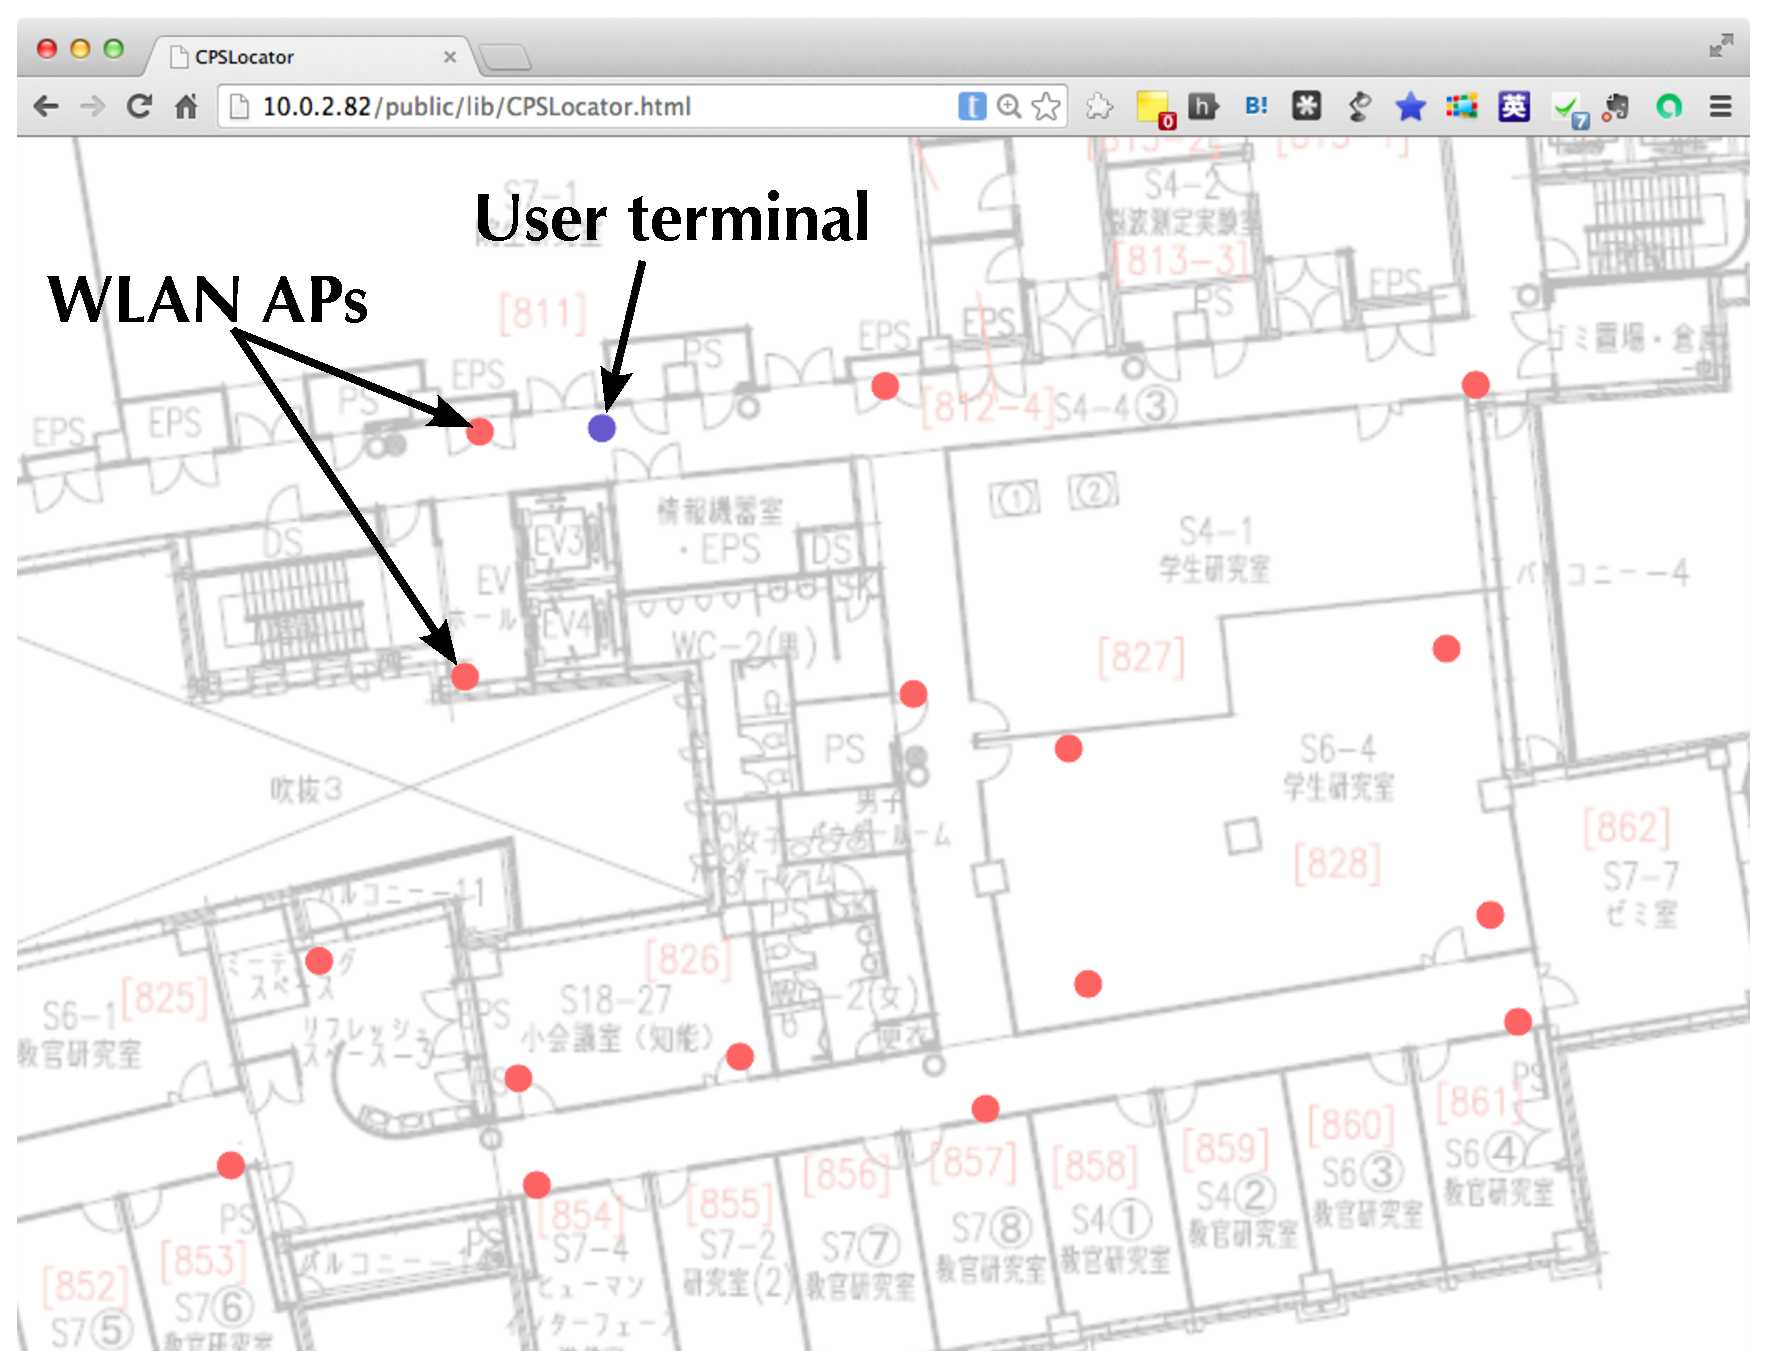
\includegraphics[width=0.8\columnwidth]{figure/map_app.eps}
 \caption{実装した屋内地図Webアプリケーション}
 \label{fig:app_screenshot}
\end{figure}

位置情報サービスの例として,屋内においてユーザ位置を表示する地図アプリケー
ションを実装した.
\figurename~\ref{fig:app_screenshot}に実装した地図アプリケーションの画面
例を示す.
屋内地図上にユーザ端末と無線LAN APの位置を表示するシンプルなWebアプリケー
ションである.

%----------------------------------------------------------------------
\section{評価}
\label{sec:eval}

\ref{sec:app-less}で示したアプリケーションレス測位システムについて実証評
価を行った.
30台のPCWLを無線LAN APとして九州大学伊都キャンパスウエスト2号館8階の廊下
や教室内に設置した.
ユーザ端末として静止状態にある1台のPCを無線LAN APの1つに接続し,PC上の
Webブラウザを用いて屋内地図Webアプリケーションのページにアクセスした.
この状態で各無線LAN APにおいてRSSI情報の受信や測位計算に関する情報を約20
分間収集した.
測位CGIにおけるRSSI情報収集の待機時間は10秒とし,125回の測位計算が記録さ
れた.

%--------------------------------------------------
\subsection{測位}

\begin{figure}[bt]
 \centering
 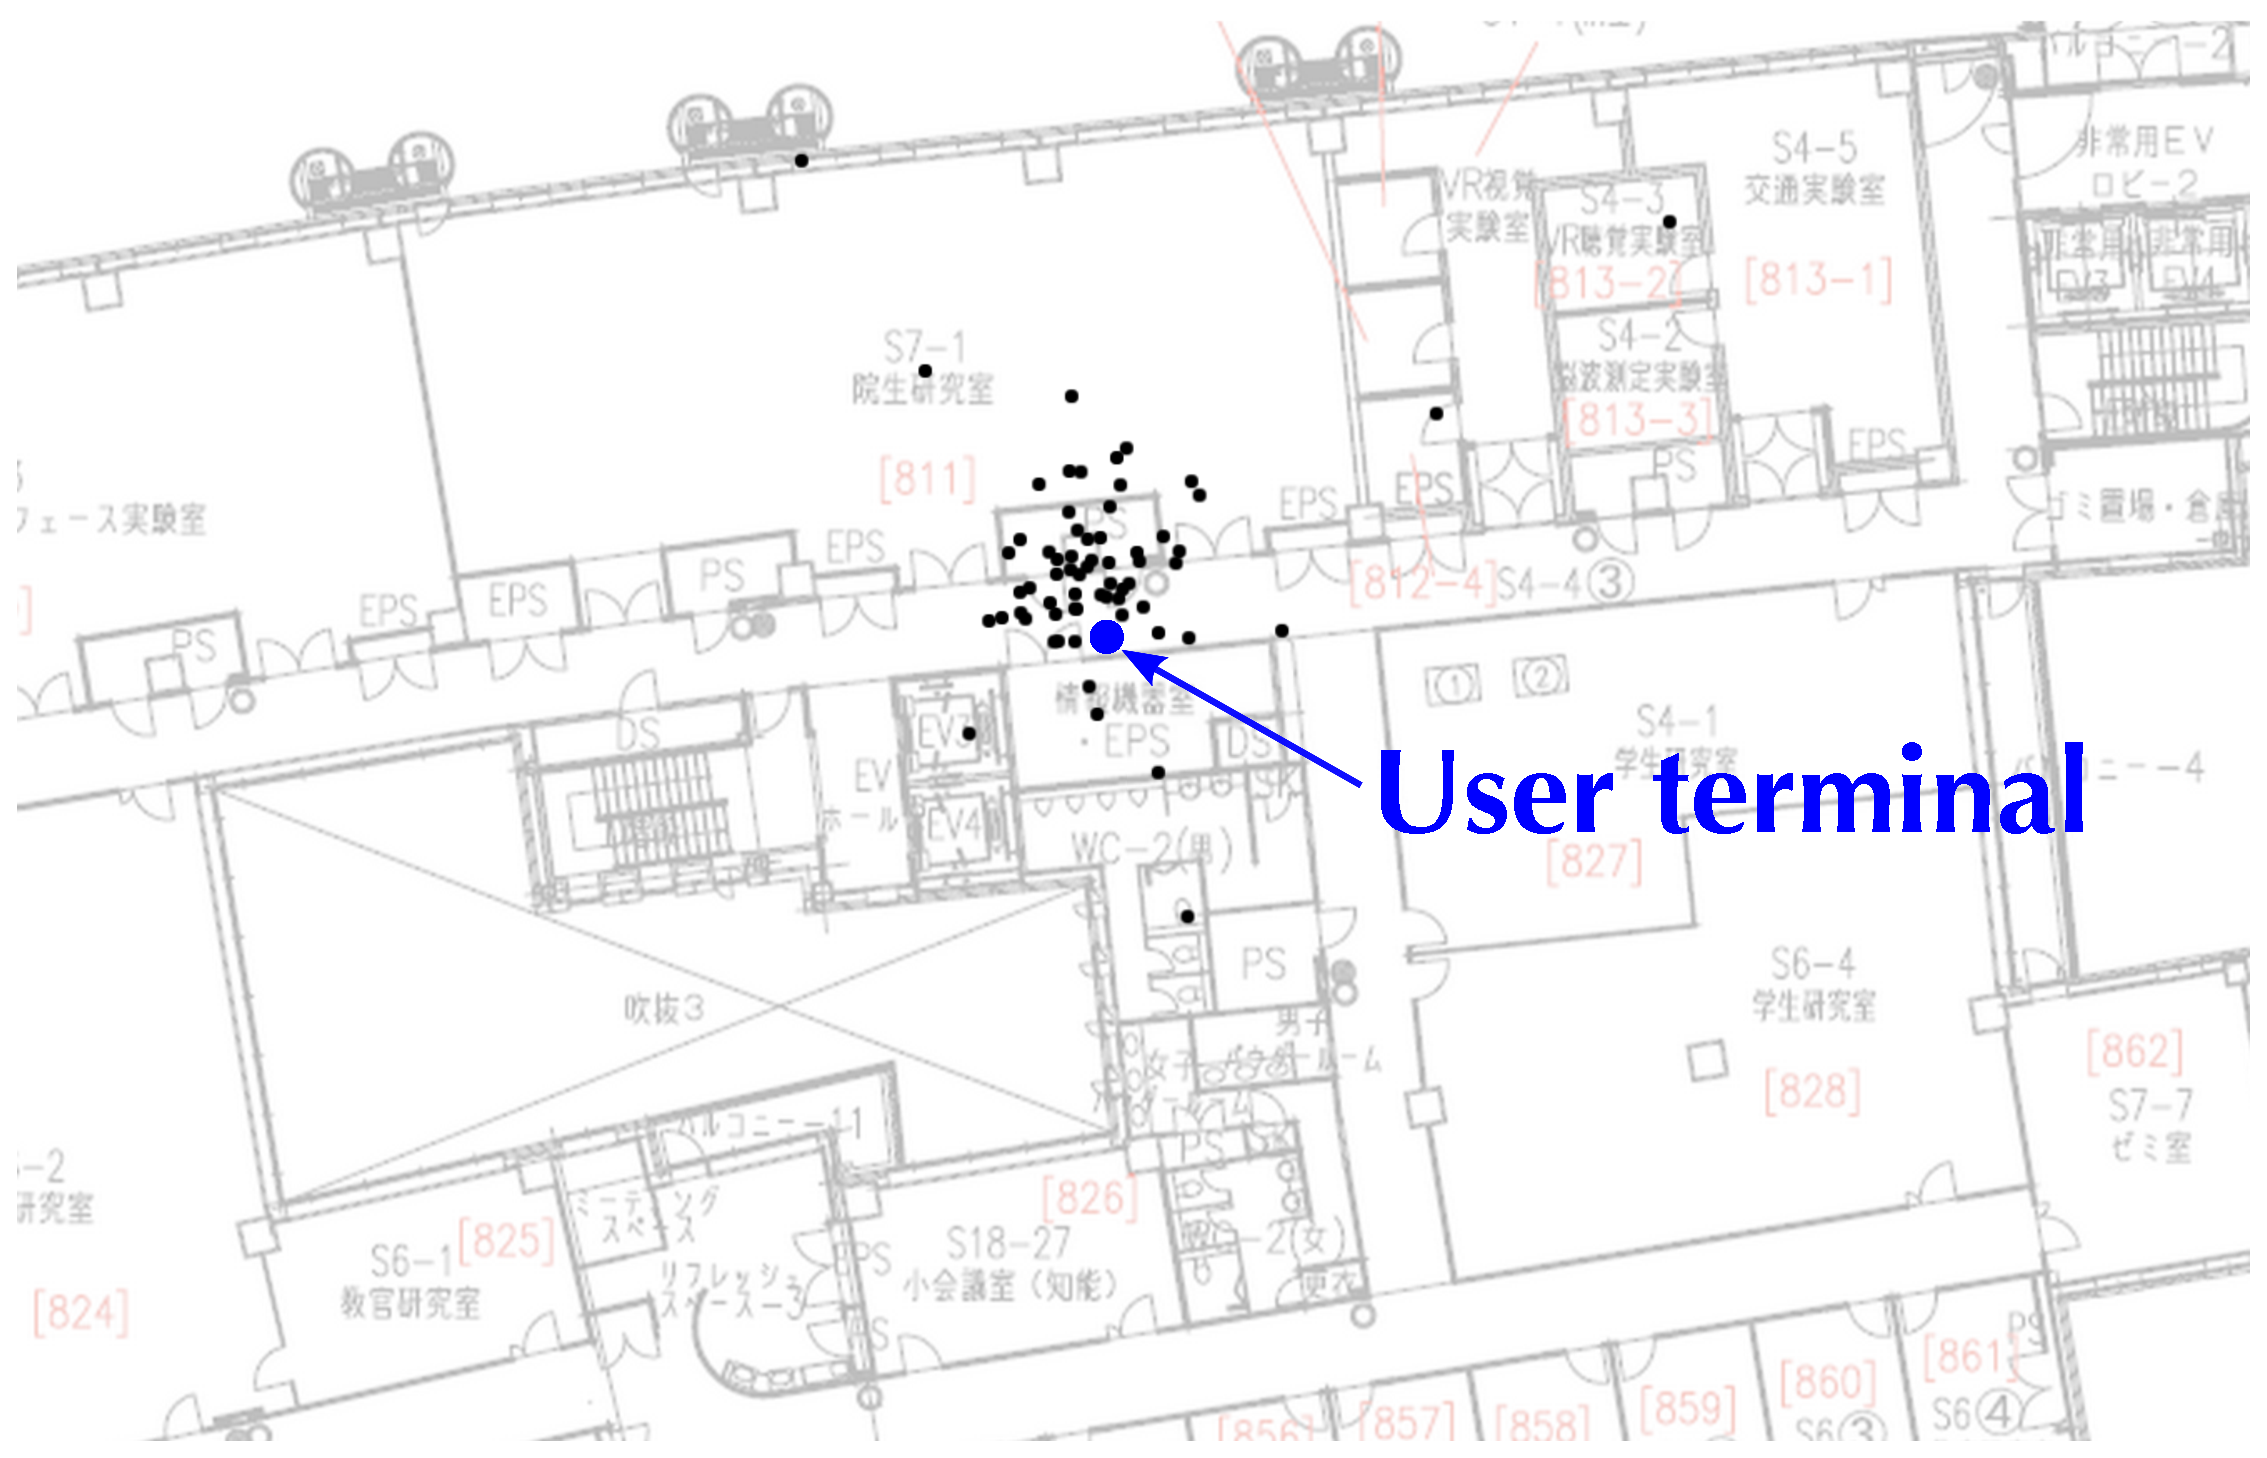
\includegraphics[width=0.8\columnwidth]{figure/positionplot.eps}
 \caption{ユーザ端末位置の測位結果}
 \label{fig:positionplot}
\end{figure}

アプリケーションレス測位システムを用いて位置情報サービスが実現できること
を示すために,測位結果を確認した.

\figurename~\ref{fig:positionplot}に本システムによって得られたユーザ端末
位置を示す.
実際のユーザ端末位置と比較すると,おおよそのユーザ端末位置を測定できてい
ることが分かる.

図に示されているように,一部の測定結果は実際のユーザ端末位置から離れた場
所を示している.
これは,測位計算に用いたアルゴリズムが,観測したRSSIに含まれる誤差によっ
て大きな測位誤差を生じたためと考えられる.

本研究は測位精度の向上を目的としていないため,測位計算においては単純な多
辺測量法を用いている.
観測したRSSIから端末位置を推定する技術に関しては多くの研究が報告されてい
るため,例えば文献\cite{izumi13:awpn_acc_imprv}などの手法を適用すること
で測位精度を向上できると考えている.

%--------------------------------------------------
\subsection{RSSI情報の送信回数}

アプリケーション測位システムにおける通信の分散は,ユーザ端末に物理的に近
い無線LAN APだけがユーザ端末の測位要求を検出することによって実現される.
これを検証するため,各無線LAN APのRSSI観測サーバが測位要求を検出した回数
を評価した.
RSSI観測サーバは測位要求を検出するとRSSI情報を送信するため,RSSI情報の送
信回数を通じて評価を行った.

\begin{figure}[bt]
 \centering
 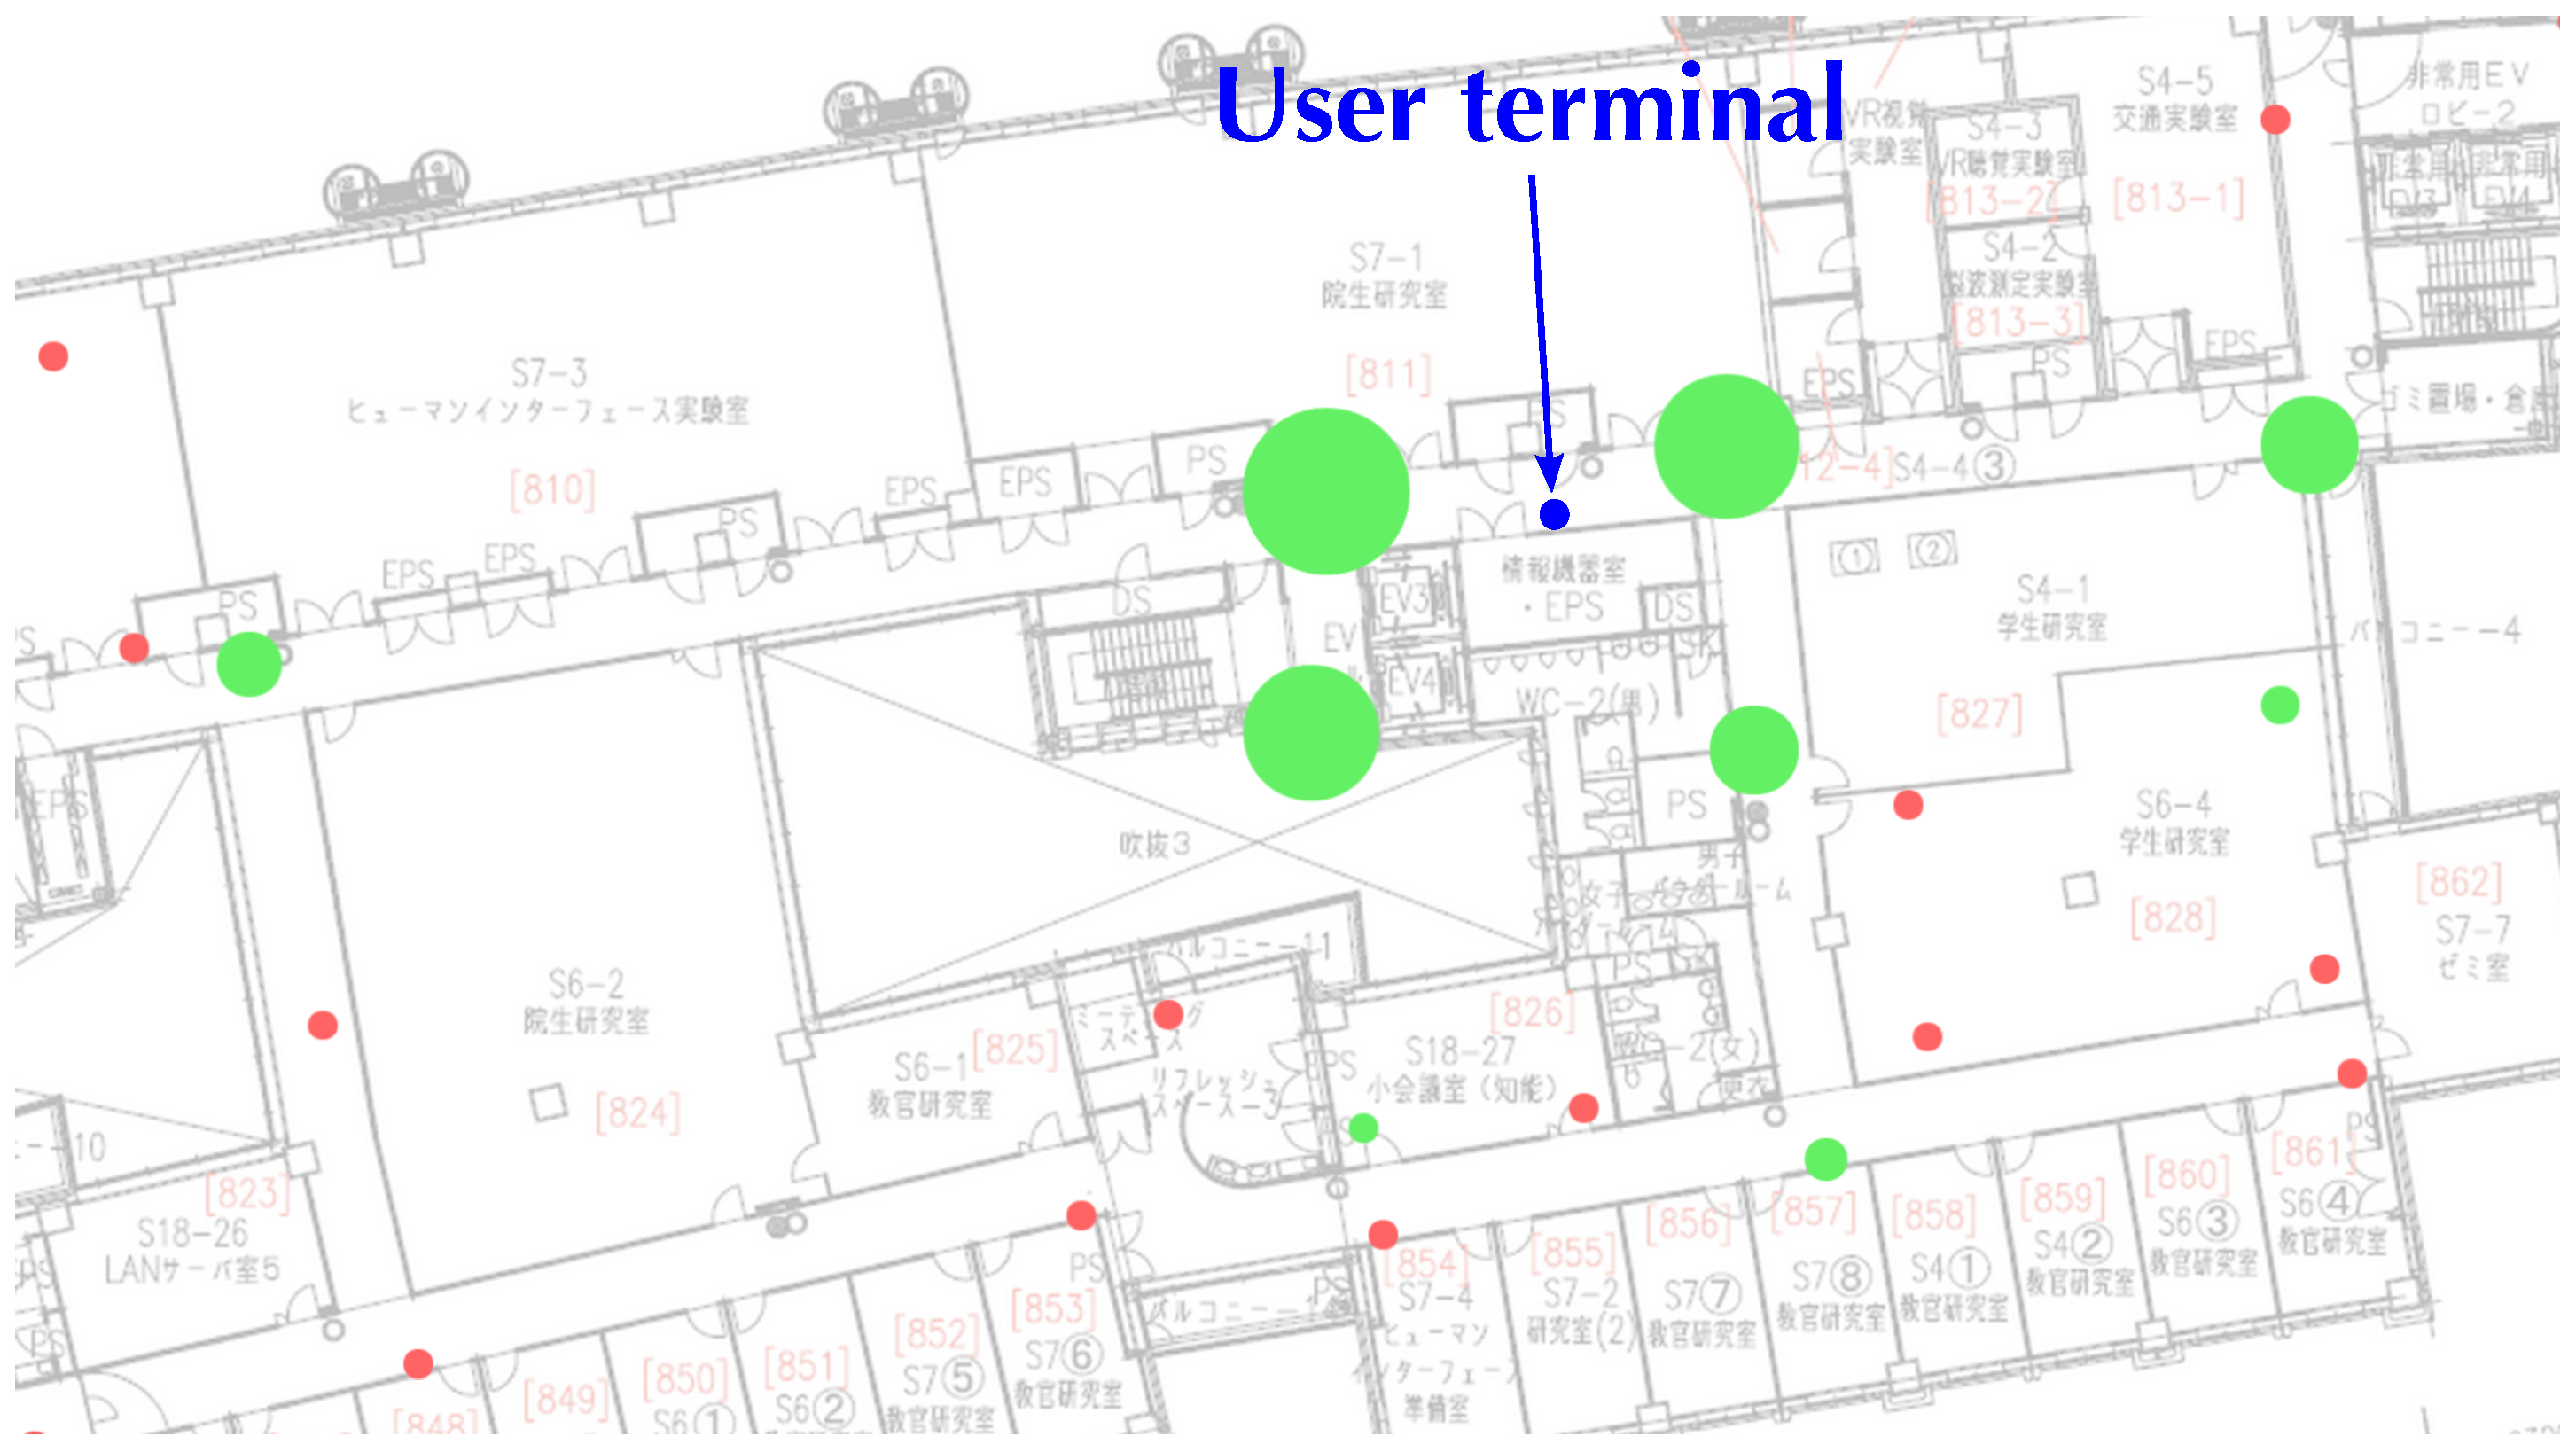
\includegraphics[width=0.8\columnwidth]{figure/catch_count.eps}
 \caption{各無線LAN APのRSSI情報送信回数}
 \label{fig:catch_count}
\end{figure}

\figurename~\ref{fig:catch_count}に各無線LAN APにおけるRSSI情報の送信回
数を示す.
図では,円の中心が無線LAN APの位置を,円の大きさがRSSI情報の送信回数を示
しており,最小・最大の円は再送を含めてそれぞれ0回,155回の送信を示してい
る.
図より,ユーザ端末に近い無線LAN APがより多くの測位要求を検出したことが分
かる.

一方,ユーザ端末から離れた位置にある無線LAN APでも測位要求を検出する場合
があることが分かる.
これは,当該無線LAN APとユーザ端末の位置が見通し距離にあるためと考えられ
る.
さらなる通信の分散に向けては,測位用無線LAN APの設置場所の検討や宛先に応
じたRSSI情報の送信有無などの手法を取り入れる必要があることが分かる.

%--------------------------------------------------
\subsection{RSSI情報の受信時間}
\label{ssec:rssi_rx_time}

\begin{figure}[bt]
 \centering
 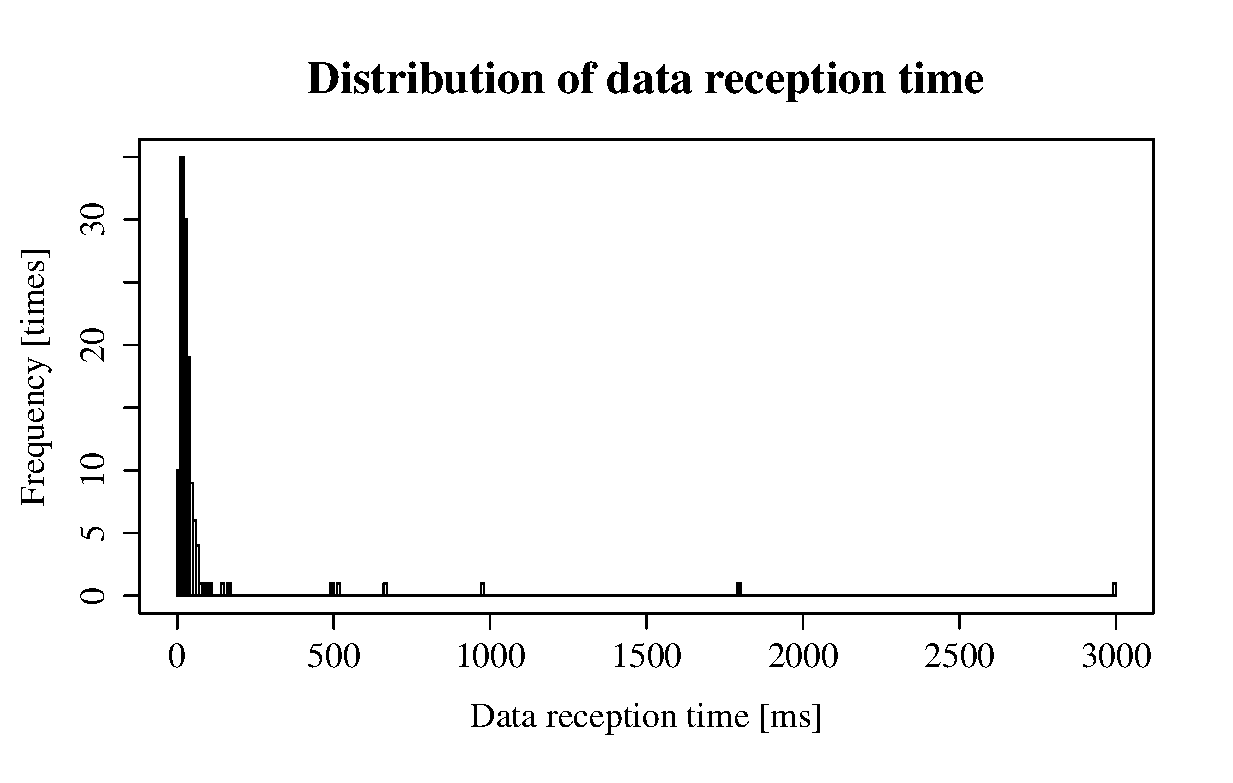
\includegraphics[width=0.8\columnwidth]{figure/recv_time.eps} \\
 (a)\\
 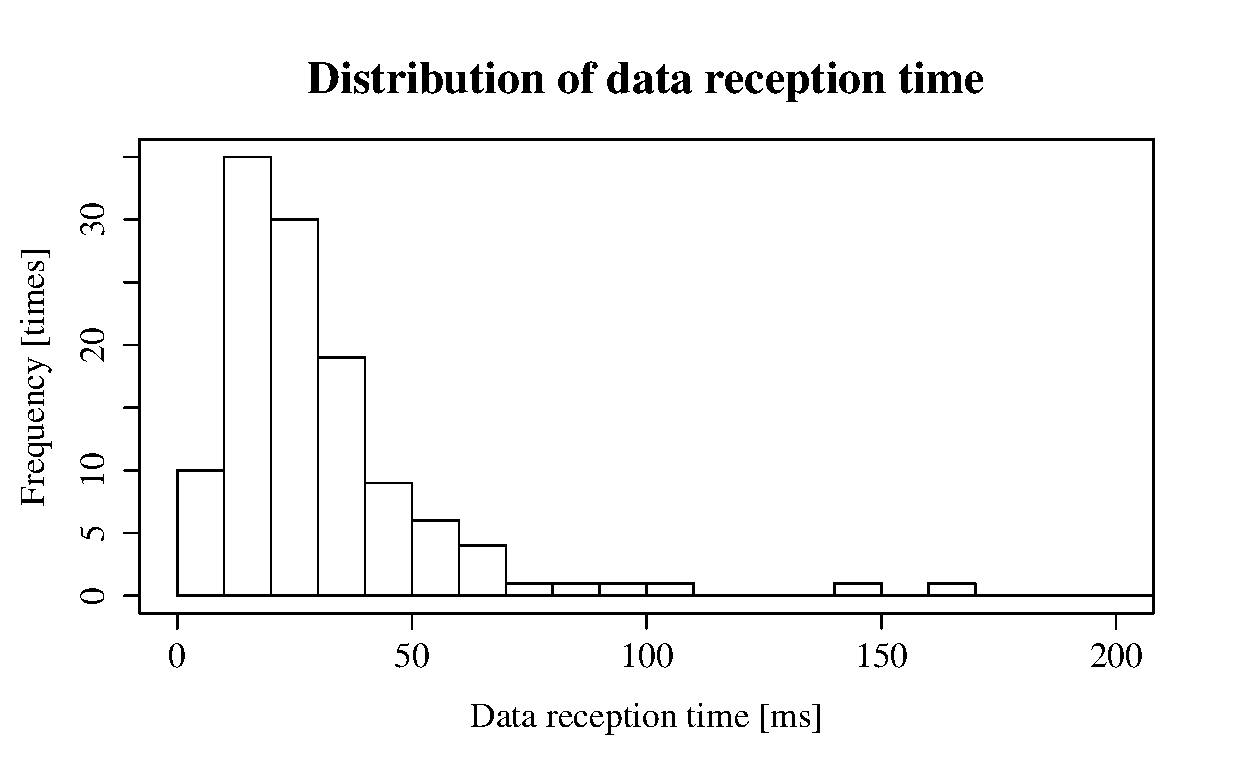
\includegraphics[width=0.8\columnwidth]{figure/recv_time_detail.eps} \\
 (b)
 \caption{RSSI情報受信時間の分布}
 \label{fig:recv_time}
\end{figure}

\ref{ssec:design_web_server}で述べたように,測位CGIはRSSI情報が収集され
るまで待機する必要がある.
待機時間の決定に向けて,RSSI情報の受信に要する時間の評価を行った.

\figurename~\ref{fig:recv_time}に各測位計算においてRSSI情報の受信に要し
た時間の分布を示す.
RSSI情報受信時間の平均値は88.8\,ms,最大値は2999.7\,msである.
\figurename~\ref{fig:recv_time}~(a)に示すように,ほとんどの測位計算におい
て200\,ms以内にRSSIの受信が完了することが分かる.
\figurename~\ref{fig:recv_time}~(b)は,同図(a)の時間軸$0\sim200$\,ms部分
を抜き出したものである.
物理的に近い無線LAN APのみに通信をとどめた結果としてほとんどの通信が
70\,ms以内に終了し,遠いAPがRSSI情報を送信した場合に遅延時間が長くなって
いると考えられる.
また,TCP通信を用いているため,転送に失敗して再送が行われた場合に200\,ms
以上の遅延が生じたと考えられる.

このような評価結果を用い,位置情報サービスの要求に従って測位CGIにおける
待機時間を決定することができる.
例えば,地図アプリケーションにおいては毎回確実に結果が得られなくても大き
な問題とはならないため,再送によって送られたRSSI情報を無視することとして
待機時間を200\,msとすればよい.

%--------------------------------------------------
\subsection{測位計算時間}

測位遅延は,測位CGIへのWebアクセスの時間を除けば測位CGIの待機時間と測位
計算時間の和となる.
測位遅延を見積もるため,測位計算時間を評価した.

\begin{figure}[bt]
 \centering
 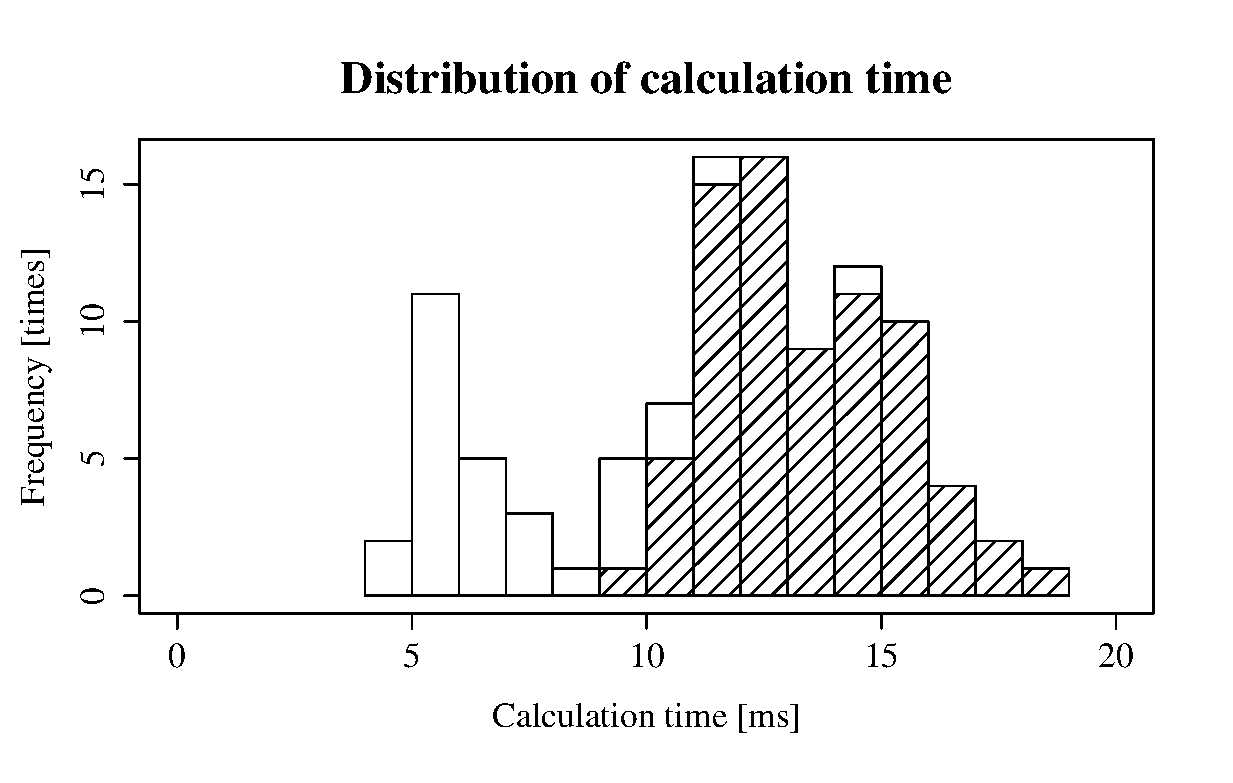
\includegraphics[width=\columnwidth]{figure/calc_time.eps}
 \caption{測位計算時間の分布}
 \label{fig:calc_time}
\end{figure}

\figurename~\ref{fig:calc_time}に各測位の計算時間の分布を示す.
白抜きは全測位,斜線は計算結果が得られたものを示している.
図より,計算時間が短いときには多くの場合において計算結果が得られないこと
が分かる.
これは,計算に必要なRSSI情報が足りない場合,あるいはRSSI情報が少なくて解
を求められないと判断した場合と考えられる.
また,計算時間が長いときにも計算結果が得られないことがあることが分かる.
十分な数のRSSI情報が得られても,RSSI値に含まれている誤差によって解が求ま
らない場合があるためと考えられる.

%%--------------------------------------------------
%\subsection{測位に用いたRSSI情報数}
%
%\begin{figure}[bt]
% \centering
% 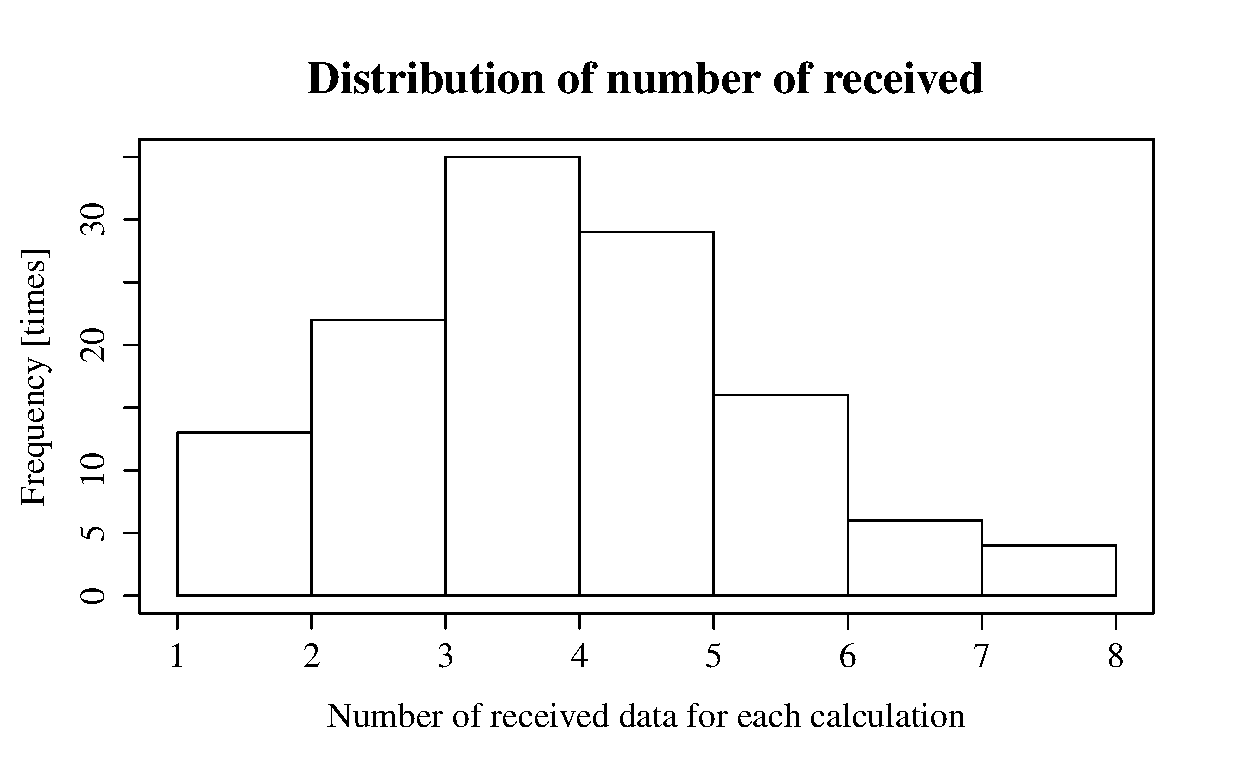
\includegraphics[width=0.8\columnwidth]{figure/recv_num.eps}
% \caption{測位に用いたRSSI情報数の分布}
% \label{fig:recv_num}
%\end{figure}
%
%無線LAN APの設置密度の検討に向けて,一度の測位において用いられたRSSI情報
%の数を評価した.
%\figurename~\ref{fig:recv_num}に各測位に用いられたRSSI情報数の分布を示す.
%平均で4.4個,最大で8個のRSSI情報を用いて測位計算が行われた.
%図より,多くの場合において$3\sim5$個のRSSI情報を用いていることが分かる.
%これは,\figurename~\ref{fig:catch_count}に示したRSSI情報の送信回数が多
%い無線LAN APがRSSI情報を送信しているためと考えられる.
%
%% 1台: 2回
%% 2台: 11回
%% 全:  125回
%125回の測位計算のうち13回はRSSI情報の数が3個未満となっている.
%測位計算に利用したアルゴリズムは3個未満のRSSI情報では測位計算を行うこと
%ができないため,測位結果を得られない.
%測位結果が得られる頻度を向上するためには,無線LAN APを設置する位置につい
%て検討が必要である.

%----------------------------------------------------------------------
\section{おわりに}
\label{sec:concl}

本稿では,一時的な位置情報サービスの実現に向けて,容易に構築可能なアドホッ
ク測位ネットワーク上でユーザがアプリケーションを導入することなく利用可能
な測位システムを示した.
位置情報サービスをWebサービスとして実現する際に問題となる通信負荷の集中
について述べ,これを解決するためにユーザ端末接続先AP内を中心とした分散型
の測位システムを示した.
本システムを無線LANメッシュノード上に実装して動作を確認するとともに基本
性能の評価を行った.
今後の課題として,ユーザ端末の集中に伴う通信負荷集中が挙げられる.
本システムではユーザ端末の物理的な位置の分散によって通信負荷を分散するた
め,ユーザ端末が集中した場合には通信負荷を分散することが困難となる.
また,測位精度向上に向けて提案されている手法を本システムのような分散測位
システム上で実現する手法について検討する必要がある.

%----------------------------------------------------------------------
% 謝辞
%----------------------------------------------------------------------
\ack
本研究の一部は,科研費(22300025,25870928) 及び文部科学省「社会システム・
サービスの最適化のためのIT統合システム構築」(採択課題名: 「社会システム・
サービス最適化のためのサイバーフィジカルIT統合基盤の研究」)の助成で行わ
れた.

%----------------------------------------------------------------------
% 参考文献
%----------------------------------------------------------------------
\bibliographystyle{sieicej}
\bibliography{bib/IEEEabrv,bib/mystr_IEICE,bib/my,bib/pub}

\end{document}
